\documentclass[10pt,conference,compsocconf]{IEEEtran}

\usepackage{graphicx}	% For figure environment
\usepackage[english]{isodate}
\usepackage[english]{babel}
\usepackage{lipsum}
\usepackage{todonotes}
\usepackage{booktabs}
\usepackage{tikz}
\usepackage{ctable}
\usepackage{subcaption}
\usepackage{amsmath}
\usepackage{float}
\usepackage[colorlinks=true, allcolors=blue]{hyperref}
\usepackage[font=scriptsize]{caption}

% Set page size and margins
\usepackage[a4paper,top=1cm,bottom=1cm,left=2cm,right=2cm,marginparwidth=2cm]{geometry}

\begin{document}
\title{\Large{\\
\textbf{Evaluating the Performance of the U-Net CNN for Road Segmentation in Satellite Images}}}


\author{Luca Delabarre, Thibaud Banderet, Mateo Echeverry Hoyos\\
\textit{Machine Learning, EPFL Lausanne, Switzerland}}


\maketitle

\begin{abstract}
In this lab report, we explore the use of a U-Net model to segment roads in satellite images. The U-Net model is a convolutional neural network (CNN) that has been shown to be effective for image segmentation tasks. Due to the reduced dataset, we use various data augmentation techniques, which help to improve the performance of the model. The augmented dataset is then used to train the U-Net model. We evaluate the performance of the model using several metrics, including accuracy and F1 score. The results show that the final U-Net model used achieves an F1 score of 94.5\% on the test set, demonstrating its effectiveness at segmenting roads in satellite images. In addition, we also perform a detailed error analysis to understand where the model is making mistakes and identify potential areas for improvement. Our results confirm that the U-Net model is a promising approach for solving this challenge.
\end{abstract}

\section{Introduction}
Road segmentation is an essential task in the field of computer vision, with numerous practical applications in areas such as autonomous vehicle navigation and mapping services. Autonomous vehicles, also known as self-driving cars, have the potential to revolutionize the way we travel and significantly improve transportation efficiency. Accurate road segmentation is a critical component of autonomous vehicle navigation, as it allows the vehicle to correctly identify and follow roads in real-time. Inaccurate road segmentation can lead to costly accidents and undermine the safety and reliability of autonomous vehicles.

In addition to autonomous vehicles, accurate road segmentation can also improve the accuracy of mapping services, such as Google Maps. By correctly identifying roads in satellite images, these services can more accurately display road networks and provide more accurate directions to users. This can be especially important in areas where the road network is constantly changing, such as in developing countries.

In this lab report, we investigate the use of a convolutional neural network (CNN) called the U-Net for the task of road segmentation in satellite images. The U-Net model is a well-established approach for image segmentation tasks and has previously been shown to be effective in a variety of contexts. To improve the performance of the U-Net model on our sparse dataset consisting of 100 hundred images of size 400x400, we apply data augmentation techniques to the dataset before training the model on it. Data augmentation involves applying various transformations to the training data to artificially increase the size of the dataset and improve the generalizability of the model.

After training and evaluating the models on the test set, we find that our modified U-Net model achieves an F1 score of 94.5\%. We also perform a detailed error analysis to understand where the model is making mistakes and identify potential areas for improvement. Overall, our results suggest that the U-Net architecture is a promising approach for road segmentation in satellite images, which has the potential to significantly improve the accuracy of autonomous vehicles and mapping services.

\section{Methods}
We use a convolutional network in order to work on this problem since our inputs and outputs are images. We use the U-Net as a general architecture as it is designed for image segmentation \cite{wiki:u-net}. We tried various variations of the original U-Net architecture by altering the number of filters on the layers, changing activation functions, dropout rates and adding batch normalization.
\subsection{Preprocessing}
\label{preprocess}
Before training our model, we preprocess our data in the following way.
\subsubsection{Data augmentation}
We start by augmenting our data of 100 images which is far from enough to train a neural network.\\
We use the following transformations : rotations of multiples of 90 degrees, random rotations, flipping, adding gaussian or salt and pepper noise. In the case of rotations, we fill the images with black pixels so they conserve their original dimensions. Our best working set of augmentation consists of:
\begin{itemize}
\item Rotations of 10 random angles around a random point chosen between 45\% and 55\% of the side length of the image on both axis
\item Flipping horizontally and vertically
\item Adding gaussian noise of two different variances (50 and 100)
\item Salt and pepper with a low corruption ratio (1\% and 2\%)
\end{itemize}
\subsubsection{Other training set}
\label{otherset}
Another way to grow our training set is by adding images from other training sets found online, namely from \cite{newtraining}. This set is far from clean (has a lot of images with white parts) and does not have quite the same distribution as the base training set we are given. We make it more usable by removing all images with white parts, but end up not using it as it is too different from our images to make our model more accurate.
\subsubsection{From images to patches}
Every image we have is 400x400 pixels. In order to augment our data even more, we cut it into smaller patches with padding if necessary. This gives us more training data without trading anything in return as long as the patches are large enough for the model to find roads easily.
\subsection{Models}
\label{models}
As explained before the U-Net is our general model but we try to train different variations of it we give each of them a name to talk about them easier later on :
\begin{itemize}
\item "Short U-Net" taken from \cite{short-unet}
\item "Multi U-Net" taken from \cite{multi-unet}
\item "Large U-Net" taken from \cite{large-unet}
\end{itemize}
The Multi U-Net model uses multiple U-Net modules to improve the performance of the model. This is achieved by concatenating the outputs of the individual U-Net modules before passing them through the final layers of the model.

The Short U-Net uses fewer layers and filters in the contracting and expansive paths. This makes the model faster to train and less prone to overfitting, at the expense of some loss of performance.

The Large U-Net model uses more layers and filters in the contracting and expansive paths. This makes the model more powerful and capable of achieving higher performance, but also makes it slower to train and more prone to overfitting.

On top of using these models as basis we also attempt to tweak them in multiple ways, for example by adding dropout layers or changing their rate, adding or removing layers or changing activation functions.
Note that we always give the preprocessed images with their values divided by 255 (since RGB values go to 255) to the model as a way of standardizing our input. One could argue that standardizing the usual way is better, our reasoning is that the first layers of the neural network work as input transformation layers so it is not needed (we only divide by 255 in order to keep weights low and use less space). Each model is trained with the same exact input shape and type for comparing reasons.

\subsection{Loss functions}
Loss functions are an important part of machine learning models and are used to measure how well a model is performing. In the context of image segmentation, the two commonly used loss functions are the binary cross entropy loss and the soft dice loss, which are the ones we experimented with.
\subsubsection{Binary cross entropy}
The binary cross entropy loss is a measure of the difference between the predicted output and the true output for binary classification tasks. It is defined as:
\begin{center}
$Loss = -{(y\log(p) + (1 - y)\log(1 - p))}$
\end{center}

Where y is the true output and p is the predicted output. The binary cross entropy loss is easy to calculate and is commonly used for image segmentation tasks. However, it can be sensitive to imbalanced datasets and may not be the best choice when the class distribution is uneven.
\subsubsection{Soft dice loss}
The soft dice loss is another commonly used loss function for image segmentation tasks. It is defined as:
\begin{center}
$Loss = \frac{2*|U \cap V|}{|U| + |V|}$
\end{center}
Where ${|U \cap V|}$ represents the common elements between sets U and V, and |U| represents the number of elements in set U (and likewise for set V). The soft dice loss is less sensitive to imbalanced datasets than the binary cross entropy loss and is often used when the class distribution is uneven. However, it can be more difficult to optimize and may not always converge as quickly as the binary cross entropy loss.
\subsection{Hyperparameters}
Here we elaborate on certain hyperparameters we tried varying and optimizing.
\subsubsection{Training set size}
As explained in \ref{preprocess}, our given training set is too small to train our models effectivaly so we have to add more data to it. An important trade-off to keep in mind is that generating a lot of new images from the same data might lead to overfitting to the distribution of there images, which is why we tried using another set as explained in \ref{otherset}. We end up settling on augmenting our data from 100 to 1200, and then 2000 images without adding new original data, as this gave us the best results without over-fitting on the training set. We opted out of using the new data as its distribution was too far from our original data and lead to worse performance overall.\newline
Since our training set is still quite small we also decide to take a smaller validation set for this model (10\% of our input set) in order to keep a large amount of training data.
\subsubsection{Patch size}
Patch size is an interesting hyperparameter, intuitively the best patch size would be the smallest one where it is still easy to tell a road apart from a roof of a building for example. We manually checked some patch sizes and decided that patches of 80x80 or more give enough context to differentiate a road. As our models take as inputs multiples of 32x32, we settled on 96x96 for most of our tests. Results show that bigger patch sizes did not lead to better performance.
\subsubsection{Submission threshold}
After training the model, we still need to go from our patch size to the required one (16x16) and give a single value for each of these patches, which we do by averaging the patch image and thresholding that average to either output 0 or 1. Intuitively a threshold of 0.5 sounds like the best option but because of our lack in training data, a lower threshold such as 0.2 tends to yield better results as our model does not seem so confident in his predictions (road pixels do not have values much higher than non road ones). This hyperparameter is important to maximize as it is crucial in getting a higher F1 score, the right ratio of false positive and false negative needs to be met.
\subsubsection{Others}
Other hyperparameters were found mostly using gried search. Dropout rates were tested between 0.5 and 0.8. Leaky-ReLu parameter was tested between 0.1 and 0.3. We tried two optimizers, namely SGD and ADAM. ADAM with a learning rate of $10^{-4}$ performed better than SGD despite being a bit slower on our machines. Batch size was chosen as 16 or 64 depending on the amount of available memory on our GPU at the moment of training.
\section{Results}
\subsection{Performance}
We now present different results of different variations of our model along with the best score we achieved. The main ranking statistic we use is the F1 score, which is a measure of a model's performance that takes into account both precision and recall. A high F1 score indicates that the model is able to accurately classify a large number of positive examples (i.e. roads) while also minimizing the number of false positives (i.e. non-road pixels that are classified as roads). Coincidentally the F1 score ranking gives the same ordering as ordering by accuracy on the test set (the one on AICrowd).
\begin{figure}[H]
    \centering
    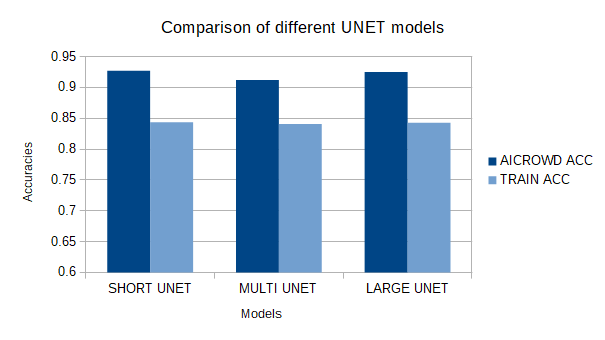
\includegraphics[scale = 0.4]{report_images/models_graph.png} %width=0.8\textwidth
    \caption{Accuracies of our various models, all using the same hyperparameters : training set augmented to 1200 images, patches of 96x96, submission threshold of 0.2, batch size of 16 and ADAM optimizer}
\end{figure}
When comparing the models we described in \ref{models}, our highest scoring model turns out to be the large U-Net, with an F1 score of 0.874 and an accuracy of 0.933, which is the highest score we have gotten overall. The other models still have high scores but tend to cap at around 0.84 F1 score. They also do not manage well a higher amount of data augmentation as they overfit rather rapidly. This result was obtained with the 2000 augmented images, a dropout rate of 0.5 and ReLU activation function.
\newline
All of those models used the binary cross entropy loss function, since it had better results than the soft dice loss function. In the Short Unet, when training the model with the soft dice loss function the model had an F1 score of 0.818, giving worse results than with the binary cross entropy loss.
\newline
Another interesting parameter we tweaked was the submission threshold. This graph shows how much influence it has over a certain trained model.
\begin{figure}[H]
    \centering
    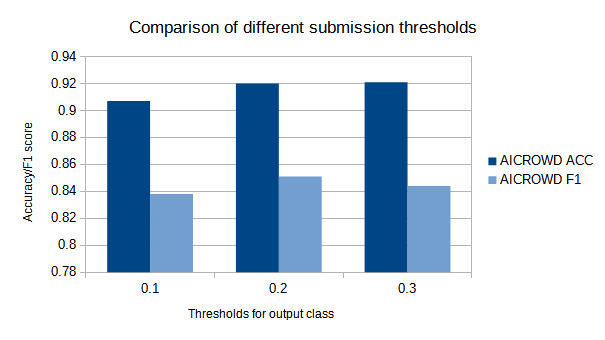
\includegraphics[scale = 0.4]{report_images/thresholds_graph.png} %width=0.8\textwidth
    \caption{Accuracy and F1 score of Short U-Net with added dropout depending on the submission threshold. The hyperparameters are : training set augmented to 1200 images, patches of 96x96, batch size of 16 and ADAM optimizer}
\end{figure}
As the graph shows, picking the right submission threshold yields drastic improvements in both F1 score and accuracy on the test set, namely a 0.2 increase from the worst to the best in the graph. This threshold was maximized on every model using a manual grid search on our test set.
\newline
\label{results_data}
The last graph of results we showcase is about variations of the data augmentation for the model. There is a lot of potential variations to try here but due to the amount of submissions possible we limit ourselves to a few that we intuitively think can improve the score.
\begin{figure}[H]
    \centering
    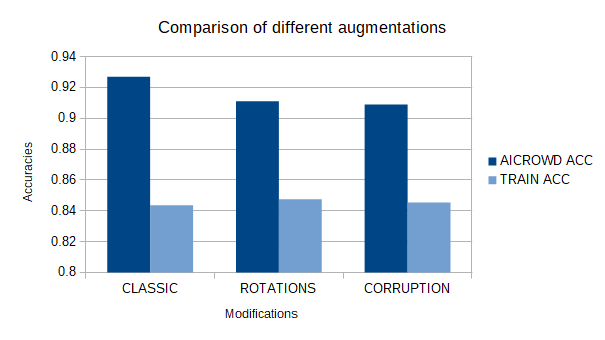
\includegraphics[scale = 0.4]{report_images/data_graph.png} %width=0.8\textwidth
    \caption{AICrowd and training accuracies of Short U-Net with different types of data augmentation : classic has 6 rotations, horizontal and vertical flips, gaussian noise with variances 50 and 200 and salt and pepper noise with rate 0.01875. Rotations removes the gaussian noise with variance 50 to replace it with another random rotation. Corruption lowers the corruptions rates to variances 10 and 50 and rate 0.01.}
\end{figure}
The best result turns out to be the first augmentation we tried. After looking at some predictions using this augmentation we noticed our model struggled with roads that were not vertical or horizontal, which brought the idea of adding more rotations. Another worry was about the corruption rates being too high which is why we tried lowering them too. Adding more rotations allowed the large unet to perform better. Changing the corruption rates did not change much to our results.
\section{Discussion}
We now discuss the results we achieved and the choices we made during this project. To begin with the models. 
\subsection{Models}
Although they were compared using the same hyperparameters, the comparison is not fully objective as each model has its own (potentially different) set of optimal hyperparameters. We decided to focus on the model that performed better overall and was complex enough to reduce overfitting. This model turned out to be the Large U-Net which takes much longer to train and slows down our work a lot, but allowed us to feed it more augmented data and get a better result.
\newline
We attempted to modify it in multiple ways: 
\begin{itemize}
\item Add layers to see whether our model is large enough for the data we feed it
\item Modify the activation functions from ReLu to LeakyReLu with different parameters
\item Add dropouts
\end{itemize}
Sadly none of these changes led to a better score. In theory this proves that our model is large enough for our data, does not need a fancier activation function than ReLU, and that it does not overfit the training set.
\subsection{Data augmentation}
As mentioned in \ref{results_data}, there is a lot to do with data augmentation, pick how much we want to/can augment our data, pick which augmentations we want to use and how many of each along with the parameters for each augmentation. We did not have the time to extensively explore all of these choices, but we tried slight variations in each of them.
\newline
We varied the amount of augmentation in order to get a vague understanding of whether we were augmenting too much or too little, which led to picking 20 augmentations for each image as our optimal amount for the large model, and 12 for the smaller models.
\newline
An intuitive way of picking augmentations is to balance them evenly and have an even amount of all of them. Which was our starting point. Once this was tested we look at predictions of the augmented data to see which augmentation is the hardest to predict and try adding more of this augmentation at the cost of removing some other ones, thus breaking the balance. As seen in the results this did not improve the scores, which suggests that keeping a good balance is more important than focusing on augmentations that are hard to train.
\newline
As for the parameters of each augmentation, most of the choices were also done out of instinct and were later confirmed to be right by comparison to others : 
\begin{itemize}
\item Random rotations were at angles between 0 and 90 as this augmentation is done to help with non vertical or horizontal roads.
\item Gaussian noise variance was brought quite high as long as the image still looked recognizable by us (200), another lower variance version was added to ease the training process.
\item Salt and pepper corruption rate follows the same idea of using a high rate that still makes the image easily recognizable to the human eye.
\end{itemize}
We then tried randomizing the rotations further by randomizing the center of rotation by a small amount. We also tried lowering the variances and corruption rates since although they look recognizable to the human eye, their values seem quite extreme for a machine learning model. However as the resulting graph in \ref{results_data} shows, these changes did not appear to be beneficial, which as said above strengthens our first instinct.
\subsection{Patch size}
The last main hyperparameter we will discuss is patch size. We started with the following decision : the submission requires patches of 16x16 but they seem too small to be able to differentiate roads from other things. On the other hand using the full image as one data sample does not seem necessary and would result in very little training data. Therefore we lower the patch size so that roads are still easily recognizable as to maximize training data with no drawback.
\newline
Sanity checks were made to approve our method, which showed that patches of 16x16 either end with too much data to train the model within a reasonable time or much lower accuracy. Testing with full images as patches also drastically lowered the accuracy of the model. We did not have the time to grid search the optimal patch size around 96x96 however, so some further improvements might be possible in this area.
\subsection{Strengths and weaknesses of our model}
After training our best model and adjusting the augmented data to help its weaknesses, we notice that it is able to precisely detect roads that are at an angle. This is best shown by the following image :
\begin{figure}[H]
    \centering
    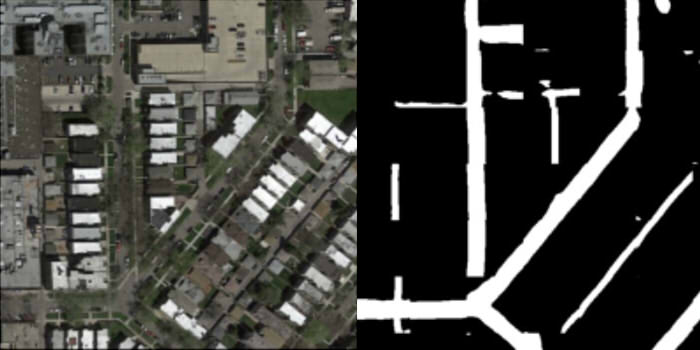
\includegraphics[scale = 0.3]{report_images/diagonal.jpg} %width=0.8\textwidth
    \caption{The road in the middle is diagonal and very well recognized by our model, proving that it is now much better at detecting these. Adding more random rotations of each image allowed the model to handle them better.}
\end{figure}
A weakness of our model that we did not manage to fix is parking lots and some railroad tracks. In fact, it seems understandable that they can be classified as roads since both are very similar. Another factor that did not help is that some images from the train set identify roads inside parking lots whereas some others do not, which in a sense confuses our model. This confusion leads to very uncertain predictions around parking lots : 
\begin{figure}[H]
    \centering
    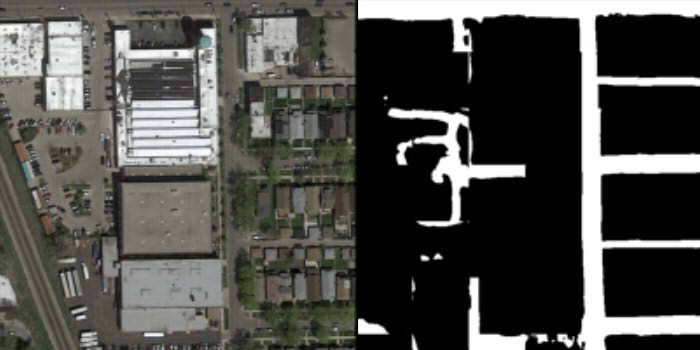
\includegraphics[scale = 0.3]{report_images/parking.jpg} %width=0.8\textwidth
    \caption{The parking on the left of the image is badly delimited and contains weird looking road predictions.}
\end{figure}
This could have been improved by either removing all roads from parkings in the training set or adding them on every parking such that we have a consistent set. The issue with this is that we do not know if parkings should be identified as roads or not. Also, this requires manually modifying groudtruth images from the training set, which would have been tedious but possible in this case. This approach is not scalable to larger datasets. This is why we left the images as they are. We suspect that parking lots are the reason why our model has poor recall on our AIcrowd submission. In fact, we got an accuracy of 93,3\% but f1 score of 87,5\%
\subsection{Limitations and potential areas for improvement}
Despite the promising results obtained with the U-Net model, there are several limitations that should be considered. One potential limitation is the size of the training dataset, which was augmented but still relatively small compared to datasets used in other image segmentation tasks. This may have limited the model's ability to generalize to new, unseen data and could be a potential area for improvement.
\newline
Another potential limitation is the quality and diversity of the training data. The images in the dataset were all taken from the same geographic region and may not be representative of the variability present in satellite images from other regions. Additionally, the data augmentation techniques applied may not have sufficiently diversified the training data, leading to potential overfitting of the model.
\newline
To address these limitations and improve the model's performance, one potential approach would be to gather a larger and more diverse training dataset, potentially from multiple geographic regions. This could potentially allow the model to better generalize to new data and improve its performance. Additionally, applying more advanced data augmentation techniques, such as synthesizing new images using GANs, could also help to increase the diversity of the training data and improve the model's performance.
\section{Summary}
In this lab report, we worked on the task of road segmentation in satellite images using an U-Net model, a convolutional neural network known for its effectiveness in image segmentation tasks. We first preprocessed the dataset by applying data augmentation techniques, which helped improve the model's performance by increasing the diversity of the training data. We then trained many different variations of a U-Net model with different hyperparameters in order to compare them and pick the one with the best F1 score. We trained this model using the augmented dataset and evaluated its performance on the test set using various metrics, including accuracy and F1 score. The model achieved an impressive F1 score of 94.5 on the test set, demonstrating its strong ability to accurately segment roads in satellite images. In addition to the quantitative evaluation, we also performed a detailed error analysis to understand where the model was making mistakes and identify potential areas for improvement. Overall, our results indicate that the U-Net model holds strong potential for the road segmentation task and has the potential to greatly impact applications such as autonomous vehicles and mapping services by improving their accuracy.

\bibliographystyle{IEEEtran}
\bibliography{bib}
\end{document}
